\subsection{Resolución de Programas Lineales}

En esta materia se ven dos métodos para resolver PPLs:
\begin{itemize}
  \item \textbf{Método Gráfico}: se basa en la representación gráfica de las restricciones y de la solución. Tiene la ventaja de ser muy intuitivo y sencillo de entender, pero tiene la desventaja de ser poco eficiente y muy limitado en cuanto al número de variables.
  \item \textbf{Método Analítico}: Es más general que el método gráfico ya que no tiene la desventaja de límite de variables. Este método se conoce como el método Simplex y es muy eficiente y algorítmico. La desventaja es que requiere la transformación previa al \textit{formato estándar} añadiendo variables de holgura y/o variables artificiales.
\end{itemize}
Más adelante veremos en profundidad los dos métodos, así que no se preocupe por el vocabulario desconocido.

\subsubsection{Típos de solución}

Todo PPL puede tener alguna de las siguientes soluciones:
\begin{itemize}
  \item Solución optima única
  \item Solución optima múltiple
  \item Problema no acotado
  \item Problema infactible
  \item Rayo óptimo
\end{itemize}

A continuación vamos a profundizar un poco sobre qué significa cada tipo de solución, para que al momento de resolver PPLs sepa identificar qué tipo de solución tiene.

\paragraph{Solución óptima única}

\noindent Es el caso más común y deseable. Existe exactamente un punto en la región factible donde la función objetivo alcanza su valor óptimo (máximo o mínimo) y presenta las siguientes características:
\begin{itemize}
  \item La función objetivo tiene una pendiente única que no es paralela a ninguna cara de la región factible
  \item Gráficamente, la línea de la función objetivo ``toca'' la región factible en un solo vértice
  \item Matemáticamente, existe un único vector \(x^*\) que optimiza la función
\end{itemize}

\paragraph{Solución óptima múltiple (infinitas soluciones óptimas)}

Existen infinitos puntos que proporcionan el mismo valor óptimo de la función objetivo. Esto ocurre cuando:
\begin{itemize}
  \item La función objetivo es paralela a una de las caras (aristas) de la región factible
  \item Todos los puntos en esa arista proporcionan el mismo valor óptimo
\end{itemize}
Este tipo de soluciones tienen las siguientes características:
\begin{itemize}
  \item Cualquier combinación convexa de dos vértices óptimos adyacentes también es óptima
  \item La solución es un segmento de línea completo en la frontera de la región factible
\end{itemize}

Si el problema tiene una solución óptima múltiple, entonces no existe una preferencia por una solución sobre otra, ya que todas son óptimas. La respuesta que usted elija darle al problema será cualquiera de las soluciones óptimas, y será considerada correcta.

\paragraph{Problema no acotado}

La función objetivo puede crecer (o decrecer) indefinidamente sin violar ninguna restricción. Estos problemas presentan las siguientes características:
\begin{itemize}
  \item La región factible se extiende infinitamente en la dirección que mejora la función objetivo
  \item No existe un valor máximo (o mínimo) finito para la función objetivo
  \item Indica generalmente un error en la formulación del problema
\end{itemize}

\ejemplo : Maximizar \(z = x_1 + x_2\) sujeto solo a \(x_1 \geq 0, x_2 \geq 0\) (sin restricciones superiores).

\paragraph{Problema infactible}

No existe ningún punto que satisfaga simultáneamente todas las restricciones del problema. Este tipo de problemas pueden ocurrir en dos casos:
\begin{itemize}
  \item Las restricciones son contradictorias entre sí
  \item El conjunto de restricciones no tiene intersección común
\end{itemize}
Y presentan las siguientes características:
\begin{itemize}
  \item La región factible está vacía
  \item No hay solución posible al problema
  \item Matemáticamente: el conjunto \(\{x : Ax \leq b, x \geq 0\} = \emptyset\)
\end{itemize}

\ejemplo : Sea el siguiente PPL:
\begin{align*}
  \text{maximizar:} \quad   &z = x_1 + x_2 \\[3pt]
  \text{sujeto a:} \quad    &x_1 + x_2 \leq 5 \\
                            &x_1 + x_2 \geq 10 \\
                            &x_1, x_2 \geq 0
\end{align*}
Estas restricciones son imposibles de satisfacer simultáneamente.

\paragraph{Rayo óptimo}

Este es un caso especial del problema no acotado donde existe una dirección específica (rayo) a lo largo de la cual la función objetivo mejora indefinidamente. Este tipo de problemas presentan las siguientes características:
\begin{itemize}
  \item Existe un punto factible \(x_0\) y una dirección \(d\) tal que \(x_0 + \lambda d\) es factible para todo \(\lambda \geq 0\)
  \item La función objetivo mejora a lo largo de esta dirección: \(c^T d > 0\) (para maximización)
  \item El rayo representa la dirección de crecimiento ilimitado
\end{itemize}
La diferencia con la solución de tipo ``no acotado'' es que el rayo óptimo especifica exactamente la dirección del crecimiento infinito, mientras que ``no acotado'' es la conclusión general.

\paragraph{Identificación en el método simplex}

En el método simplex, la identificación de los tipos de soluciones se realiza de la siguiente manera:
\begin{itemize}
  \item \textbf{Única/Múltiple:} Se identifica en la tabla final del simplex
  \item \textbf{No acotado:} Aparece cuando una variable no básica tiene coeficientes no positivos en su columna
  \item \textbf{Infactible:} Se detecta cuando aparecen variables artificiales con valor positivo en la solución final
  \item \textbf{Rayo óptimo:} Se determina por la dirección correspondiente a la variable que causa el comportamiento no acotado
\end{itemize}

Cada tipo de solución tiene implicaciones importantes para la interpretación y aplicación práctica del modelo de optimización. De momento no se preocupe por entender el método simplex, ya que se verá en detalle en la siguiente sección.

\subsubsection{Método Gráfico}

Como se mencionó anteriormente, el método gráfico es muy intuitivo, y por ende, ideal para aprender los conceptos de PPLs. Para entender el método gráfico lo más sencillo es analizarlo con un ejemplo.

\ejemplo\label{ej:mtd_grfico}: Un expendio de carnes de la cuidad acostumbra a preparar carne para albondigón con una combinación de carne molida de res y carne molida de cerdo. La carne de res contiene \(80\%\) de carne y \(20\%\) de grasa, y le cuesta a la tienda \textcent \textit{80} por libra; la carne de cerdo contiene \(68\%\) de carne y \(32\%\) de grasa y cuesta \textcent \textit{60} por libra 

¿Qué cantidad de cada tipo de carne debe emplear la tienda en cada libra de albondigón, si se desea minimizar el costo y mantener el contenido de grasa no mayor al \(25\%\)?

\noindent\textbf{Resolución del ejemplo \ref{ej:mtd_grfico}:}
\begin{quote}
  \textbf{1. Identificación de variables de decisión:}
  Vemos que el resultado es un albondigón, y este se prepara con \(x_1\) libras de carne de res y \(x_2\) libras de carne de cerdo. Por lo que las variables de decisión son:
  \begin{itemize}
    \item \(x_1 ~\rightarrow\) cantidad de carne de res por libra de albondigón
    \item \(x_2 ~\rightarrow\) cantidad de carne de cerdo por libra de albondigón
  \end{itemize}

  \textbf{2. Identificación de restricciones:}
  Vemos que la cantidad total de grasa del albondigón debe ser menor o igual al 25\%, y que la cantidad de carne de res más la cantidad de carne de cerdo debe ser igual a 1 libra.

  Sumado a esto, también se tiene que las cantidades de carne de res y carne de cerdo no pueden ser negativas. Entonces, resulta:

  \begin{align*}
    0.2x_1 + 0.32x_2 &\leq 0.25 \\
    x_1 + x_2 &= 1 \\
    x_1, x_2 &\geq 0
  \end{align*}

  \textbf{3. Identificación de la función objetivo:}

  Vemos que la función objetivo es el costo total, que es la suma del costo de la carne de res y la carne de cerdo. Por lo que la función objetivo es:
  \[
    z = 80x_1 + 60x_2
  \]

  \textbf{4. Formulación del PPL:}

  Juntando la función objetivo con las restricciones, resulta en el siguiente PPL:
  \begin{align*}
    \text{minimizar:} \quad   &z = 80x_1 + 60x_2 \\[3pt]
    \text{sujeto a:} \quad    &0.2x_1 + 0.32x_2 \leq 0.25 \\
                              &x_1 + x_2 = 1 \\
                              &x_1, x_2 \geq 0
  \end{align*}

  \textbf{5. Resolución del PPL:}

  Para resolver el PPL usando el método gráfico, debemos graficar las restricciones, la región factible y la función objetivo. 

  \noindent ¿Cómo se realiza la gráfica de la función objetivo? 

  Para realizar la gráfica de la función objetivo debemos establecer un valor para el costo, y verificar si se encuentra en la región factible. Por ejemplo, nosotros vamos a elegir un valor inicial de \(z = 50\), y resolver la ecuación \(50 = 80x_1 + 60x_2\) para obtener la ecuación de la recta que representa la función objetivo.
  \begin{align*}
    50 &= 80x_1 + 60x_2 \\
    x_2 &= -\frac{4}{3}x_1 + \frac{5}{6}
  \end{align*}
  Y listo, ahora solo debemos graficar las restricciones e identificar la región factible, que la marcaremos de color \textcolor{cyan}{cyan}. 
    
  \begin{figure}[ht]
  \centering
  \begin{tikzpicture}
  \begin{axis}[
      xlabel={$x_1$},
      ylabel={$x_2$},
      xmin=0, xmax=1.5,
      ymin=0, ymax=1.2,
      grid=major,
      axis lines=center,
      legend pos=north east,
      width=10cm,
      height=8cm
  ]

  % Restricción 1: 0.2x1 + 0.32x2 <= 0.25
  \addplot[orange, thick, domain=0:1.25, name path=A] {-(4/7)*x + (5/7)};
  \addlegendentry{\(0.2x_1 + 0.32x_2 \leq 0.25\)}

  % Restricción 2: x1 + x2 <= 1
  \addplot[blue, thick, domain=0:1, name path=B] {1-x};
  \addlegendentry{\(x_1 + x_2 = 1\)}

  % Función objetivo (para un valor de z=50): 50 = 80x1 + 60x2
  \addplot[teal, thick, domain=0:1, name path=C] {-(4/3)*x + (5/6)};
  \addlegendentry{\(50 = 80x_1 + 60x_2\)}

  % Restricciones de no negatividad
  \addplot[black, thick, domain=0:10, name path=D] {0};
  \addplot[black, thick] coordinates {(0,0) (0,10)};

  % % Región factible para la restricción 1 sombreada
  % \addplot[orange!30, opacity=0.3] fill between[
  %     of=A and D,
  %     soft clip={domain=0:1.25}
  % ];

  % Región factible
  \addplot[cyan, ultra thick , domain=2/3:1, name path=E] {1-x};

  % Puntos vértices de la región factible
  \addplot[only marks, mark=*, mark size=3pt, color=black] 
  coordinates {(1,0) (2/3,1/3)};

  % Etiquetas de los vértices
  \node at (axis cs:1,0) [above right] {B (1,0)};
  \node at (axis cs:2/3,1/3) [above right] {A \(\left(\frac{2}{3},\frac{1}{3}\right)\)};

  \end{axis}
  \end{tikzpicture}
  \caption{Gráfico del PPL}
  \label{fig:ppl}
  \end{figure}

  \noindent En el gráfico se puede observar que la región factible es el segmento color cyan. En este caso, el valor de costo \(z=50\) no se encuentra dentro de la región factible. Buscar este valor a prueba y error no es lo más conveniente, entonces vamos a usar un teorema que nos asegura que la solución óptima se encuentra en un vértice del \textbf{polígono} de la región factible. Más adelante se verá la demostración de este teorema.

  Entonces, basado en el teorema, la solución óptima se encuentra en el vértice \textit{A} o en el vértice \textit{B}. A simple vista en el gráfico podemos ver que la función objetivo está más cerca del origen de coordenadas en el punto \textit{A} y por lo tanto el costo será menor, sin embargo veremos el costo en ambos puntos para mostrar que el costo aumenta a medida que la función objetivo se aleja del origen de coordenadas.

  \begin{align*}
    z_A &= 80\left(\frac{2}{3}\right) + 60\left(\frac{1}{3}\right) \\
    z_A &= \frac{220}{3} \approx \boxed{73.33} \\[5pt]
    z_B &= 80(1) + 60(0) = 80
  \end{align*}

  \textbf{6. Respuesta:} 

  En base a la resolución del PPL, se debe emplear \({2}/{3}\) de carne de res y \({1}/{3}\) de carne de cerdo por libra de albondigón para mantener el contenido de grasa no mayor al 25\%, y que el costo sea el menor posible, que es \$\(73.33\).

\end{quote}

\hrule
\vspace{5mm}

\paragraph{Resolución Bónus}

\ejemplo\label{ej:resolucion_ppl_petroleos_grafico}: Resolución del PPL del problema de la compañía de petróleos. 
\begin{quote}
  \textbf{1. Formulación del PPL:}

  A continuación se mostrará la resolución del ejercicio visto en el ejemplo \ref{ej:modelo_de_ppl_verbal}. Recordando el PPL ya modelado, se tiene:
  \begin{align*}
    \text{maximizar:} \quad   &z = 103x_1 + 110x_2 \\[3pt]
    \text{sujeto a:} \quad    &7x_1 + 10x_2 \leq 1400 \\
                              &12x_1 + 8x_2 \leq 2000 \\
                              &8x_1 + 10x_2 \geq 900 \\
                              &6x_1 + 7x_2 \geq 300 \\
                              &5x_1 + 4x_2 \geq 800 \\
                              & 5x_1 + 4x_2 \leq 1700 \\
                              &x_1 \geq 0 \\
                              &x_2 \geq 0
  \end{align*}

  \textbf{2. Resolución gráfica:}

  En este caso se tienen muchas más restricciones que en el ejemplo \ref{ej:mtd_grfico}, sin embargo siempre se terminará formando un polígono, donde los vertices indicarán las posibles soluciones óptimas. Para facilitar la resolución gráfica, escribiremos las restricciones en la forma de ecuaciones y reordenaremos los términos de cada ecuación para que queden en la forma de \(y = mx + b\).
  \begin{align*}
    7x_1 + 10x_2 = 1400 \quad &\rightarrow \quad x_2 = -\frac{7}{10}x_1 + 140 \\
    12x_1 + 8x_2 = 2000 \quad &\rightarrow \quad x_2 = -\frac{3}{2}x_1 + 250 \\
    8x_1 + 10x_2 = 900  \quad &\rightarrow \quad x_2 = -\frac{4}{5}x_1 + 90
  \end{align*}

  \begin{align*}
    6x_1 + 7x_2 = 300  \quad &\rightarrow \quad x_2 = -\frac{6}{7}x_1 + \frac{300}{7} \\
    5x_1 + 4x_2 = 800  \quad &\rightarrow \quad x_2 = -\frac{5}{4}x_1 + 200 \\
    5x_1 + 4x_2 = 1700 \quad &\rightarrow \quad x_2 = -\frac{5}{4}x_1 + 425 \\
  \end{align*}
  Y para las restricciones de no negatividad, sabemos que la región factible se tiene que encontrar el el primer cuadrante.

  Por último, antes de graficar, vamos a suponer algún valor de ganancia de la función objetivo, por ejemplo \(z = 17000\), y resolver la ecuación \(17000 = 103x_1 + 110x_2\) para obtener la ecuación de la recta que representa la función objetivo.
  \[
    17000 = 103x_1 + 110x_2 \quad \rightarrow \quad x_2 = -\frac{103}{110}x_1 + \frac{1700}{11}
  \]

  Entonces, el gráfico de la región factible y la función objetivo con la ganancia \(z = 17000\) es el siguiente:
  \begin{figure}[ht]
    \centering
    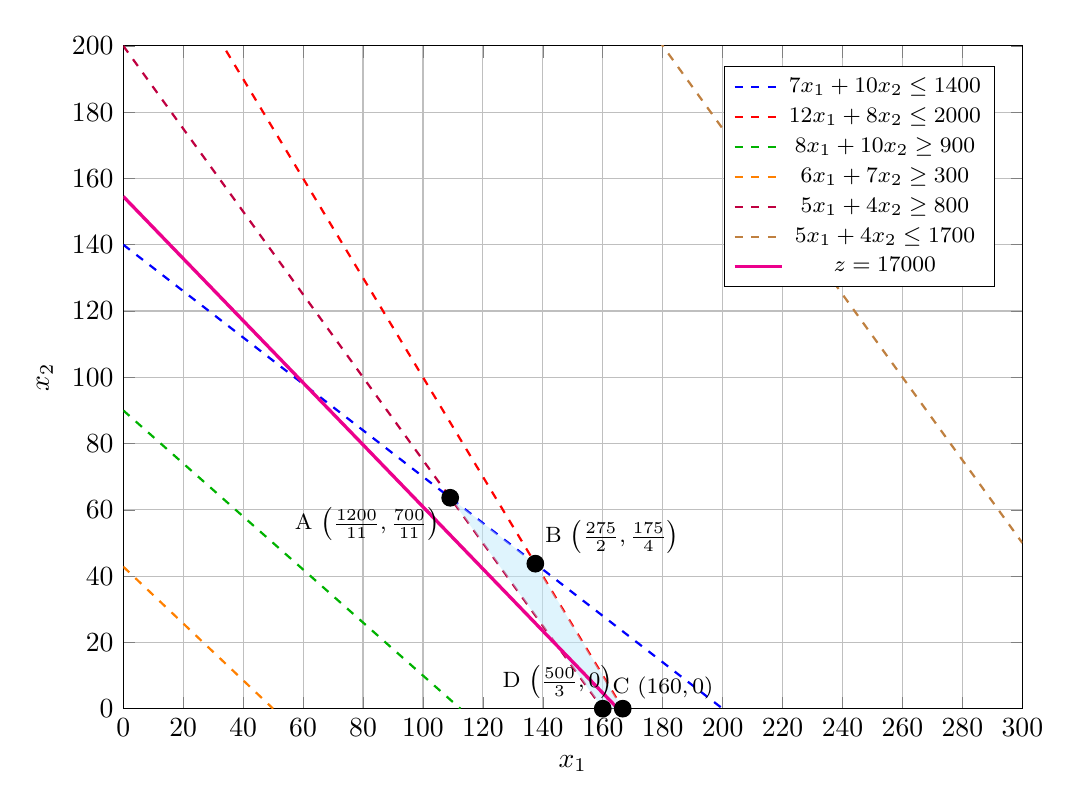
\begin{tikzpicture}
    \begin{axis}[
        xlabel={$x_1$},
        ylabel={$x_2$},
        xmin=0, xmax=300,
        ymin=0, ymax=200,
        grid=major,
        legend pos=north east,
        width=13cm,
        height=10cm,
        legend style={font=\footnotesize}
    ]
    
    % Restricción 1: 7x₁ + 10x₂ ≤ 1400 → x₂ ≤ 140 - 0.7x₁
    \addplot[blue, thick, dashed, domain=0:200] {140-0.7*x};
    \addlegendentry{$7x_1 + 10x_2 \leq 1400$}
    
    % Restricción 2: 12x₁ + 8x₂ ≤ 2000 → x₂ ≤ 250 - 1.5x₁
    \addplot[red, thick, dashed, domain=0:166.67] {250-1.5*x};
    \addlegendentry{$12x_1 + 8x_2 \leq 2000$}
    
    % Restricción 3: 8x₁ + 10x₂ ≥ 900 → x₂ ≥ 90 - 0.8x₁
    \addplot[green!70!black, thick, dashed, domain=0:112.5] {90-0.8*x};
    \addlegendentry{$8x_1 + 10x_2 \geq 900$}
    
    % Restricción 4: 6x₁ + 7x₂ ≥ 300 → x₂ ≥ 42.86 - 0.857x₁
    \addplot[orange, thick, dashed, domain=0:50] {(300/7)-(6/7)*x};
    \addlegendentry{$6x_1 + 7x_2 \geq 300$}
    
    % Restricción 5: 5x₁ + 4x₂ ≥ 800 → x₂ ≥ 200 - 1.25x₁
    \addplot[purple, thick, dashed, domain=0:160] {200-1.25*x};
    \addlegendentry{$5x_1 + 4x_2 \geq 800$}
    
    % Restricción 6: 5x₁ + 4x₂ ≤ 1700 → x₂ ≤ 425 - 1.25x₁
    \addplot[brown, thick, dashed, domain=0:300] {425-1.25*x};
    \addlegendentry{$5x_1 + 4x_2 \leq 1700$}
    
    % Región factible aproximada (necesitarías calcular los vértices exactos)
    % Esta es una aproximación visual de la región factible
    \fill[cyan!25, opacity=0.5] 
        (1200/11,700/11) -- (275/2,43.75) -- (500/3,0) -- (160,0) -- cycle;

    % Función objetivo
    \addplot[magenta, very thick, domain=0:165] {-(103/110)*x + (1700/11)};
    \addlegendentry{$z = 17000$}
    
    % Algunos puntos de intersección importantes (aproximados)
    \addplot[only marks, mark=*, mark size=3pt, color=black] 
    coordinates {(1200/11,700/11) (275/2,43.75) (500/3,0) (160,0)};
    
    % Etiquetas para algunos puntos clave
    \node at (axis cs:1200/11,700/11) [below left] {\footnotesize A \(\left(\frac{1200}{11},\frac{700}{11}\right)\)};
    \node at (axis cs:275/2,43.75) [above right] {\footnotesize B \(\left(\frac{275}{2},\frac{175}{4}\right)\)};
    \node at (axis cs:160,0) [above right] {\footnotesize C \(\left(160,0\right)\)};
    \node at (axis cs:500/3,0) [above left] {\footnotesize D \(\left(\frac{500}{3},0\right)\)};
    \end{axis}
    \end{tikzpicture}
    \caption{Región factible del PPL de ejemplo \ref{ej:modelo_de_ppl_verbal} en color \textcolor{cyan}{cyan}}
    \label{fig:ppl-maximizacion}
  \end{figure}

  Vemos que la la función objetivo \(z\) se encuentra dentro de la región factible, sin embargo, no es la solución óptima. Se puede ver que el punto más alejado del origen de coordenadas que puede tomar la función objetivo es el vértice \textit{B}. Por lo tanto, la solución óptima es el vértice \textit{B}, que es el punto \(\left(275/2,175/4\right)\). Entonces:
  \[
    z_B = 103\left(\frac{275}{2}\right) + 110\left(\frac{175}{4}\right) = \boxed{18975}
  \]

  \textbf{3. Respuesta:}

  En base a la resolución del PPL, se deben realizar \(137.5\) sesiones de destilación usando la tecnología nueva (\(T_n\)) y \(43.75\) sesiones de destilación usando la tecnología antigua (\(T_a\)), para obtener la mayor ganancia posible, que es \$\(18975\).

  \begin{tcolorbox}[remember]
    Aunque la respuesta pueda resultar confusa, recordemos que el enunciado decía que los procesos de destilación \textit{se pueden utilizar total o parcialmente}, por lo que la respuesta toma valores fraccionarios. Si se quisiera que la respuesta fuera un número entero, entonces se agregan las respectivas restricciones y se resuelve el PPL de la misma manera, tomando únicamente los puntos enteros de \(x_1\) y \(x_2\).
  \end{tcolorbox}

\end{quote}

\subsubsection{Introducción al método Simplex}

Como anteriormente mencionamos, el método simplex es un algoritmo que nos permite resolver problemas de optimización lineal. Aunque disponemos del método gráfico, cuando el número de \textit{variables de decisión} es grande (\(> 2\)), el método gráfico es impracticable, por lo que utilizar el método analítico se vuelve una necesidad.

Además, en general, la mayoría de los problemas de optimización suelen tener más de dos variables de decisión, por lo que la necesidad de generalizar la búsqueda de la solución optima es un tema de interés.

\paragraph{¿Qué hace el método Simplex?}

El método Simplex es un algoritmo iterativo que parte de una solución básica factible (es decir, un vértice del conjunto factible del problema) y se \hl{desplaza de un vértice a otro adyacente}, mejorando en cada paso el valor de la función objetivo, hasta que no se puede mejorar más, lo que significa que se ha llegado a la \textbf{solución óptima}.

Visualmente, imagina un poliedro (la región factible), donde cada vértice es una posible solución básica. El Simplex camina por los bordes del poliedro en dirección ascendente (en problemas de maximización) hasta llegar al punto más alto.

\paragraph{Estructura general del método}

El método se basa en representar el problema en \textbf{forma tabular}. Cada paso del algoritmo consiste en:
\begin{enumerate}
  \item \textbf{Iniciar en una solución básica factible inicial}: esta primera solución se obtiene en la \textit{Fase I} del Simplex. 
  \item \textbf{Seleccionar una variable entrante}: mediante la \textit{regla del criterio} se selecciona aquella que más mejora la función objetivo
  \item \textbf{Seleccionar una variable saliente}: para mantener la factibilidad (cumplir restricciones)
  \item \textbf{Actualizar la tabla (pivoteo)}: para generar una nueva solución básica
  \item \textbf{Repetir el proceso}: hasta que no haya más mejoras posibles
\end{enumerate} 
No se preocupe por entender el concepto de \textit{Fase I} y la \textit{regla del criterio}, ya que se explicarán en detalle más adelante.

\begin{tcolorbox}[interesting_data, title=Forma tabular]
  Que el método Simplex se base en representar el problema en ``forma tabular'' significa que todas las ecuaciones (la función objetivo y las restricciones) del problema de Programación Lineal se organizan en una matriz estructurada, una tabla, llamada ``tableau Simplex''
\end{tcolorbox}

Ahora, vamos a ver algunos conceptos necesarios para comprender la formulación del método, pero el método en sí se verá en el la sección \ref{sec:simplex}, ya que es bastante largo.

\vspace{3mm}

\paragraph{Forma matricial de un PPL}

Un PPL puede ser representado en forma matricial de la siguiente manera:
\begin{align*}
  \text{optimizar:} \quad   &z = C^TX \\[3pt]
  \text{sujeto a:} \quad    &AX \thicksim  B \\
\end{align*}
donde:
\begin{itemize}
  \item \(C\) es la matriz (o el vector) de coeficientes de la función objetivo, generalmente se le llama vector de costos, ya que cada coeficiente representa el costo de una variable de decisión. En la formula se denota como \(C^T\) para indicar que es una matriz transpuesta,
  \item \(X\) es la matriz (o el vector) de variables de decisión. Este vector debe incluir todas las variables del PPL, tanto las variables de decisión originales como las agregadas (como variables de holgura, superfluas, etc que se verán más adelante),
  \item \(A\) es la matriz de coeficientes de las restricciones,
  \item \(B\) es la matriz (o el vector) de términos independientes de las restricciones.
\end{itemize}
\vspace{5pt}
\noindent De forma explícita se puede ver como:
\begin{align*}
  \text{optimizar:} \quad   &z = c_{1}x_{1} + c_{2}x_{2} + \cdots + c_{n}x_{n} \\[3pt]
  \text{sujeto a:} \quad    &a_{11}x_{1} + a_{12}x_{2} + \cdots + a_{1n}x_{n} \thicksim b_{1} \\[3pt]
                            &a_{21}x_{1} + a_{22}x_{2} + \cdots + a_{2n}x_{n} \thicksim b_{2} \\[3pt]
                            &\quad \vdots \\[3pt]
                            &a_{m1}x_{1} + a_{m2}x_{2} + \cdots + a_{mn}x_{n} \thicksim b_{m}
\end{align*}
donde:
\[
  C = \begin{pmatrix} c_1 \\ c_2 \\ \vdots \\ c_n \end{pmatrix},\ X = \begin{pmatrix} x_1 \\ x_2 \\ \vdots \\ x_n \end{pmatrix},\ A = \begin{pmatrix} a_{11} & a_{12} & \cdots & a_{1n} \\ a_{21} & a_{22} & \cdots & a_{2n} \\ \vdots & \vdots & \ddots & \vdots \\ a_{m1} & a_{m2} & \cdots & a_{mn} \end{pmatrix},\ B = \begin{pmatrix} b_1 \\ b_2 \\ \vdots \\ b_m \end{pmatrix}
\]

Esta forma es conveniente ya que permite representar el PPL de una manera más compacta y permite referirnos a una parte específica del problema, como la matriz de los coeficientes (\(A\)) para referirnos a las restricciones, el vector de costos (\(C\)) para referirnos a los coeficientes de la función objetivo y el vector de términos independientes (\(B\)) para referirnos a los términos independientes de las restricciones.

Con estos conceptos estamos listos para ver la forma de resolución de PPLs mediante el método Simplex.